\documentclass[tikz,border=0pt]{standalone}
% 只引入一个最常用的 calc 库用于计算坐标，其他全是基础命令
\usetikzlibrary{calc}

% 你的品牌色
\definecolor{HypoPrimary}{HTML}{0969DA}
\definecolor{HypoAccent}{HTML}{8E44AD}

\begin{document}
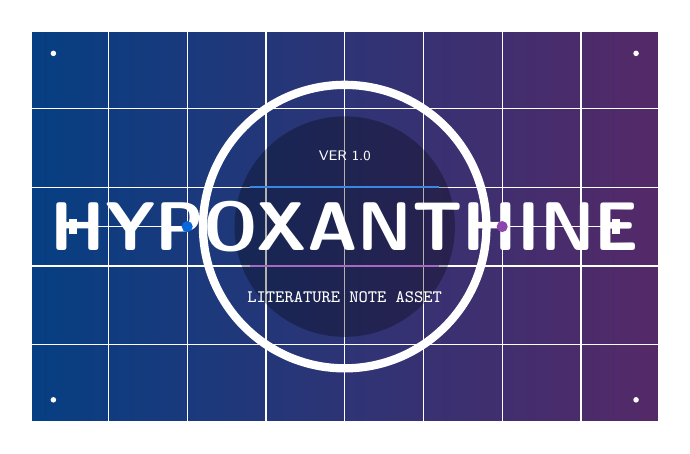
\begin{tikzpicture}
    % =========================================
    % 1. 背景层：深色渐变 + 极简网格
    % =========================================
    % 定义画布大小 8x5
    \shade[left color=HypoPrimary!60!black, right color=HypoAccent!60!black] (0,0) rectangle (8,5);
    
    % 绘制淡淡的网格
    \draw[white!5, step=1.0, line width=0.5pt] (0,0) grid (8,5);
    \draw[white, line width=1.5pt] (0,0) rectangle (8,5); % 外边框

    % =========================================
    % 2. 核心几何结构 (绝对居中)
    % =========================================
    \coordinate (Center) at (4,2.5);

    % 外部大圆环 (半透明白色)
    \draw[white!10, line width=3pt] (Center) circle (1.8);
    \draw[white!30, line width=0.8pt] (Center) circle (1.8);

    % 内部实心圆背景
    \fill[black, opacity=0.3] (Center) circle (1.4);
    
    % 上下分割线 (装饰)
    \draw[HypoPrimary!80!white, thick] ($(Center) + (-1.2, 0.5)$) -- ($(Center) + (1.2, 0.5)$);
    \draw[HypoAccent!80!white, thick]  ($(Center) + (-1.2, -0.5)$) -- ($(Center) + (1.2, -0.5)$);

    % =========================================
    % 3. 文字内容 (Hypoxanthine)
    % =========================================
    % 主标题：大写、粗体、白色
    \node[white, font=\sffamily\bfseries\Huge] at (Center) {HYPOXANTHINE};
    
    % 副标题：稍微拉开字间距
    \node[white!70, font=\ttfamily\scriptsize, scale=0.9] at ($(Center) + (0, -0.9)$) {LITERATURE NOTE ASSET};

    % 顶部版本号
    \node[white!40, font=\sffamily\tiny] at ($(Center) + (0, 0.9)$) {VER 1.0};

    % =========================================
    % 4. 对称装饰 (左右平衡)
    % =========================================
    % 左侧装饰块
    \fill[white!20] (0.5, 2.4) rectangle (0.6, 2.6);
    \draw[white!40] (0.6, 2.5) -- (2.0, 2.5);
    \fill[HypoPrimary] (2.0, 2.5) circle (2pt);

    % 右侧装饰块
    \fill[white!20] (7.4, 2.4) rectangle (7.5, 2.6);
    \draw[white!40] (6.0, 2.5) -- (7.4, 2.5);
    \fill[HypoAccent] (6.0, 2.5) circle (2pt);

    % 四角的小点缀
    \fill[white!50] (0.3, 0.3) circle (1pt);
    \fill[white!50] (7.7, 0.3) circle (1pt);
    \fill[white!50] (0.3, 4.7) circle (1pt);
    \fill[white!50] (7.7, 4.7) circle (1pt);

\end{tikzpicture}
\end{document}